% =====================================================================
%  BÁO CÁO KỸ THUẬT: TÌM HIỂU MÔ HÌNH NVIDIA ISAAC GR00T N1.7
%  Biên dịch: latexmk -xelatex Nvidia_groot.tex   (hoặc compile.cmd / watch.cmd)
%  Quy ước viết: thuật ngữ kỹ thuật giữ nguyên tiếng Anh, giải thích một lần
%  trong Bảng thuật ngữ ở đầu báo cáo; trong thân bài không mở ngoặc giải thích.
% =====================================================================
\documentclass[12pt,a4paper,oneside]{report}

\usepackage{fontspec}
\setmainfont{Times New Roman}
\setmonofont{Consolas}[Scale=0.9]
\usepackage[english,vietnamese]{babel}

\usepackage[top=2.5cm,bottom=2.5cm,left=3cm,right=2cm,headheight=15pt]{geometry}
\usepackage{setspace}
\onehalfspacing
\setlength{\parindent}{1cm}
\setlength{\parskip}{4pt}
\usepackage{indentfirst}

\usepackage{graphicx}
\graphicspath{{figures/}}
\usepackage{amsmath,amssymb}
\usepackage{booktabs}
\usepackage{array}
\usepackage{caption}
\captionsetup{font=small,labelfont=bf}
\usepackage{enumitem}
\setlist{nosep,itemsep=3pt}
\usepackage{xcolor}
\definecolor{navy}{HTML}{1F3864}
\usepackage{titlesec}
\usepackage{fancyhdr}
\usepackage{url}
\usepackage[hidelinks]{hyperref}
\hypersetup{pdftitle={Tìm hiểu mô hình NVIDIA Isaac GR00T N1.7},pdfauthor={Nguyễn Duy Hoàng}}
\sloppy
\setlength{\emergencystretch}{3em}

\titleformat{\chapter}[hang]{\normalfont\Large\bfseries\color{navy}}{\thechapter.}{0.6em}{}
\titlespacing*{\chapter}{0pt}{0pt}{18pt}
\titleformat{\section}{\normalfont\large\bfseries\color{navy}}{\thesection.}{0.6em}{}
\titleformat{\subsection}{\normalfont\normalsize\bfseries\itshape}{\thesubsection.}{0.6em}{}

\pagestyle{fancy}
\fancyhf{}
\rhead{\small\itshape Báo cáo kỹ thuật: Tìm hiểu mô hình NVIDIA Isaac GR00T N1.7}
\cfoot{\thepage}
\renewcommand{\headrulewidth}{0.4pt}
\fancypagestyle{plain}{\fancyhf{}\cfoot{\thepage}\renewcommand{\headrulewidth}{0pt}}

\newcolumntype{L}[1]{>{\raggedright\arraybackslash}p{#1}}
\newcommand{\code}[1]{\texttt{#1}}

\begin{document}

% =====================================================================
%  FRONT COVER
% =====================================================================
\begin{titlepage}
\centering
\vspace*{0.5cm}
{\large\bfseries [TÊN CÔNG TY / ĐƠN VỊ]\par}
{\bfseries [Tên nhóm / phòng ban]\par}
\vspace{4cm}
{\Large\bfseries\color{navy} BÁO CÁO KỸ THUẬT\par}
\vspace{0.8cm}
{\huge\bfseries\color{navy} TÌM HIỂU MÔ HÌNH\\[0.3cm] NVIDIA ISAAC GR00T N1.7\par}
\vspace{0.8cm}
{\large\itshape Kiến trúc, dữ liệu huấn luyện, so sánh với các mô hình cùng loại và kết quả thử nghiệm trên robot Unitree G1\par}
\vfill
{\large Người thực hiện: \textbf{Nguyễn Duy Hoàng}\par}
\vspace{0.3cm}
{\large Người nhận: [Tên mentor / quản lý]\par}
\vspace{3cm}
{\large\bfseries Tháng 9 năm 2026\par}
\vspace{0.5cm}
\end{titlepage}

% =====================================================================
%  TITLE PAGE
% =====================================================================
\pagenumbering{roman}
\begin{center}
\vspace*{1.5cm}
{\LARGE\bfseries\color{navy} TÌM HIỂU MÔ HÌNH NVIDIA ISAAC GR00T N1.7\par}
\vspace{0.6cm}
{\large\itshape Kiến trúc, dữ liệu huấn luyện, so sánh với các mô hình cùng loại và kết quả thử nghiệm trên robot Unitree G1\par}
\vspace{1.5cm}
\begin{tabular}{L{4.2cm}L{10.5cm}}
\toprule
\textbf{Mục} & \textbf{Nội dung}\\
\midrule
Loại tài liệu & Báo cáo kỹ thuật nội bộ\\
Đối tượng tìm hiểu & Mô hình \code{nvidia/GR00T-N1.7-3B} và bộ điều khiển toàn thân GEAR-SONIC của NVIDIA\\
Mục đích & Nắm cách mô hình hoạt động ở mức tổng thể, biết nó khác gì và hơn kém gì so với các mô hình cùng loại, và đánh giá khả năng dùng cho bài toán của nhóm\\
Người thực hiện & Nguyễn Duy Hoàng\\
Người nhận & [Tên mentor / quản lý]\\
Mã nguồn tham chiếu & Isaac-GR00T (commit \code{51d4c89}); GR00T-WholeBodyControl v1.1; dự án nội bộ GEAR-SONIC-GR00T-N1.7\\
Thời gian & Tháng 9 năm 2026\\
\bottomrule
\end{tabular}
\end{center}
\clearpage

% =====================================================================
%  ABSTRACT
% =====================================================================
\chapter*{TÓM TẮT}
\addcontentsline{toc}{chapter}{Tóm tắt}

GR00T N1.7 là mô hình Vision-Language-Action mã nguồn mở của NVIDIA, phát hành năm 2026, khoảng 3 tỉ tham số. Mô hình nhận ảnh camera, câu lệnh bằng lời và trạng thái khớp của robot, rồi trả về 40 bước hành động tiếp theo. Bên trong gồm hai khối: một khối VLM để hiểu ảnh và câu lệnh, một khối Diffusion Transformer để sinh hành động. Với robot hình người, mô hình không điều khiển trực tiếp từng khớp mà đưa ra một token chuyển động 64 chiều, rồi bộ điều khiển toàn thân GEAR-SONIC giải mã token này thành lệnh cho 29 khớp ở 50\,Hz và tự lo giữ thăng bằng.

Báo cáo trình bày cách mô hình hoạt động ở mức các tầng chính, không đi sâu vào toán; so sánh GR00T N1.7 với $\pi_{0.5}$ và các mô hình cùng loại; chỉ ra điểm mạnh, điểm chưa ổn, và vì sao cách tiếp cận này tốt hơn policy lập trình sẵn hay policy học một nhiệm vụ. Phần kết quả ghi lại ba việc nhóm đã làm: nối GR00T N1.7 với bộ điều khiển toàn thân trên mô phỏng MuJoCo của Unitree G1; tự sinh dữ liệu demo cho nhiệm vụ phân loại lon Coca-Cola và Pepsi; và fine-tune mô hình trên Google Colab. Kết quả open-loop trên 40 episode kiểm tra cho sai số MAE 0,0053 theo đơn vị chuẩn hoá, tương đương khoảng 0,3 độ, chênh lệch train-test khoảng 3\%. Thử nghiệm closed-loop và mở rộng dữ liệu là việc đang làm tiếp.

\noindent\textbf{Từ khoá:} \textit{Vision-Language-Action, GR00T N1.7, Diffusion Transformer, whole-body control, GEAR-SONIC, Unitree G1, fine-tuning.}
\clearpage

% =====================================================================
%  TOC
% =====================================================================
\renewcommand{\contentsname}{MỤC LỤC}
\tableofcontents
\clearpage

% =====================================================================
%  BẢNG THUẬT NGỮ
% =====================================================================
\chapter*{BẢNG THUẬT NGỮ}
\addcontentsline{toc}{chapter}{Bảng thuật ngữ}
Báo cáo giữ nguyên thuật ngữ tiếng Anh trong thân bài. Nghĩa của từng thuật ngữ ghi ở bảng này và không nhắc lại.

\begin{center}\small
\begin{tabular}{L{4cm}L{10.6cm}}
\toprule
\textbf{Thuật ngữ} & \textbf{Nghĩa}\\
\midrule
VLM & Vision-Language Model: mạng hiểu cả ảnh và văn bản, cho ra vector đặc trưng chung.\\
VLA & Vision-Language-Action: VLM mở rộng để đầu ra là hành động robot thay vì văn bản.\\
Backbone & Khối VLM lớn nằm ở đầu mô hình, thường được tái sử dụng từ mô hình có sẵn.\\
Action head & Khối nằm sau backbone, chuyên sinh hành động.\\
DiT & Diffusion Transformer: Transformer sinh dữ liệu bằng cách khử nhiễu dần.\\
Flow matching & Cách huấn luyện khử nhiễu đơn giản hơn diffusion cổ điển, cần rất ít bước khi chạy.\\
Token & Một vector đại diện cho một mẩu dữ liệu: một ô ảnh, một từ, một bước hành động.\\
Attention & Cơ chế cho các token trao đổi thông tin với nhau.\\
Cross-attention & Attention giữa hai nhóm token khác nhau, ví dụ token hành động hỏi token ảnh.\\
Action chunk & Một đoạn nhiều bước hành động tương lai được dự đoán trong một lần chạy.\\
Embodiment & Hình thái vật lý của một robot: số khớp, kiểu tay, camera. Mỗi loại robot là một embodiment.\\
Proprioception & Trạng thái tự cảm nhận của robot: góc khớp, vận tốc, hướng thân.\\
End-effector, EEF & Điểm cuối của tay máy, thường là cổ tay hoặc bàn tay.\\
Relative action & Hành động ghi dưới dạng độ dời so với trạng thái hiện tại, thay vì mục tiêu tuyệt đối.\\
Whole-body control, WBC & Điều khiển đồng thời toàn bộ khớp của robot hình người, gồm cả giữ thăng bằng.\\
GEAR-SONIC & Bộ điều khiển toàn thân của NVIDIA cho Unitree G1, nhận token chuyển động và trả lệnh khớp.\\
Motion token & Vector 64 chiều mô tả một ý định chuyển động, do SONIC định nghĩa.\\
Fine-tune & Huấn luyện thêm một mô hình có sẵn trên dữ liệu của mình.\\
Open-loop, closed-loop & Open-loop: so hành động dự đoán với dữ liệu ghi sẵn. Closed-loop: cho mô hình điều khiển thật và xem có hoàn thành nhiệm vụ không.\\
Policy & Hàm ánh xạ từ quan sát sang hành động; VLA là một dạng policy.\\
LeRobot & Định dạng dataset robot của Hugging Face mà GR00T dùng.\\
\bottomrule
\end{tabular}
\end{center}
\clearpage

% =====================================================================
%  PHẦN II
% =====================================================================
\pagenumbering{arabic}
\setcounter{page}{1}

% ---------------------------------------------------------------------
\chapter{GIỚI THIỆU}
% ---------------------------------------------------------------------
\textcolor{gray}{\itshape [Phần này do tác giả tự viết. Gợi ý: bài toán của nhóm, lý do chọn GR00T N1.7, câu hỏi cần trả lời cho mentor, cấu trúc báo cáo.]}

% ---------------------------------------------------------------------
\chapter{CƠ SỞ LÝ THUYẾT}
% ---------------------------------------------------------------------
Chương này chỉ nêu bốn ý cần có để đọc chương 3 và 4.

\section{Vision-Language Models và VLA}

VLM là mạng đọc được cả ảnh và chữ: ảnh bị cắt thành các ô, mỗi ô thành một token, rồi token ảnh và token chữ cùng đi qua một mô hình ngôn ngữ để trộn thông tin với nhau. VLA lấy VLM làm phần hiểu cảnh và gắn thêm một action head để cho ra hành động robot. Mỗi lần chạy, VLA trả về một action chunk gồm nhiều bước tương lai; robot thực thi một phần rồi hỏi lại.

\section{Diffusion Models và Diffusion Transformer}

Cùng một cảnh có nhiều cách gắp đúng, nên nếu bắt mạng đoán thẳng một hành động thì nó sẽ đoán ra ``trung bình'' của các cách, thường là sai. Diffusion bắt đầu từ nhiễu và khử nhiễu dần thành một quỹ đạo cụ thể, tức là chọn một cách thay vì lấy trung bình. Flow matching là bản gọn của diffusion, chỉ cần vài bước khi chạy. DiT là cách làm bằng Transformer: mỗi bước hành động là một token, các token trao đổi với nhau và hỏi thông tin từ ảnh, chữ qua attention.

\section{Robotic Manipulation và Whole-Body Control}

Với tay máy, ghi hành động ở EEF dưới dạng relative action giúp mô hình bớt phụ thuộc vị trí tuyệt đối và cho phép dùng chung cách ghi giữa tay người trong video và tay robot. Với robot hình người, thao tác luôn đi cùng thăng bằng, nên hệ thống chia hai tầng: VLA chạy vài Hz quyết định làm gì, WBC chạy 50\,Hz quyết định từng khớp và giữ robot không ngã. Giao diện giữa hai tầng là điểm mấu chốt.

\section{Tổng quan các phiên bản GR00T và mô hình liên quan}

\begin{itemize}
\item \textbf{GR00T N1} (3/2025): VLA mở đầu tiên của NVIDIA cho robot hình người, 2,2 tỉ tham số.
\item \textbf{GR00T N1.5} (6/2025): đóng băng backbone, nghe lệnh tốt hơn.
\item \textbf{GR00T N1.6} (cuối 2025): DiT 32 lớp, thêm tag \code{UNITREE\_G1\_SONIC} cho WBC.
\item \textbf{GR00T N1.7} (2026, bản chính thức): backbone Cosmos-Reason2-2B; relative action ở EEF chung cho người và robot; thêm 20 nghìn giờ video người; chunk 40 bước; xuất ONNX, TensorRT; dùng thương mại được.
\end{itemize}

Mô hình cùng loại: $\pi_0$, $\pi_{0.5}$ của Physical Intelligence, OpenVLA; về phía WBC là GEAR-SONIC của NVIDIA. Chương 5 so sánh.

% ---------------------------------------------------------------------
\chapter{KIẾN TRÚC MÔ HÌNH}
% ---------------------------------------------------------------------
Số liệu trong chương lấy từ mã nguồn Isaac-GR00T và checkpoint \code{GR00T-N1.7-3B}. Một vài tham số có hai giá trị: mặc định trong mã nguồn và giá trị thật trong checkpoint; báo cáo ghi giá trị của checkpoint vì đó là thứ chạy khi fine-tune.

\section{Kiến trúc tổng thể}

Hệ thống của nhóm gồm hai mô hình độc lập ghép lại: GR00T N1.7 quyết định làm gì, GEAR-SONIC quyết định từng khớp quay thế nào. Mục này mô tả pipeline của từng mô hình khi đứng riêng, rồi pipeline chung khi ghép.

\subsection{Pipeline của NVIDIA GR00T N1.7}

\begin{figure}[htbp]
\centering
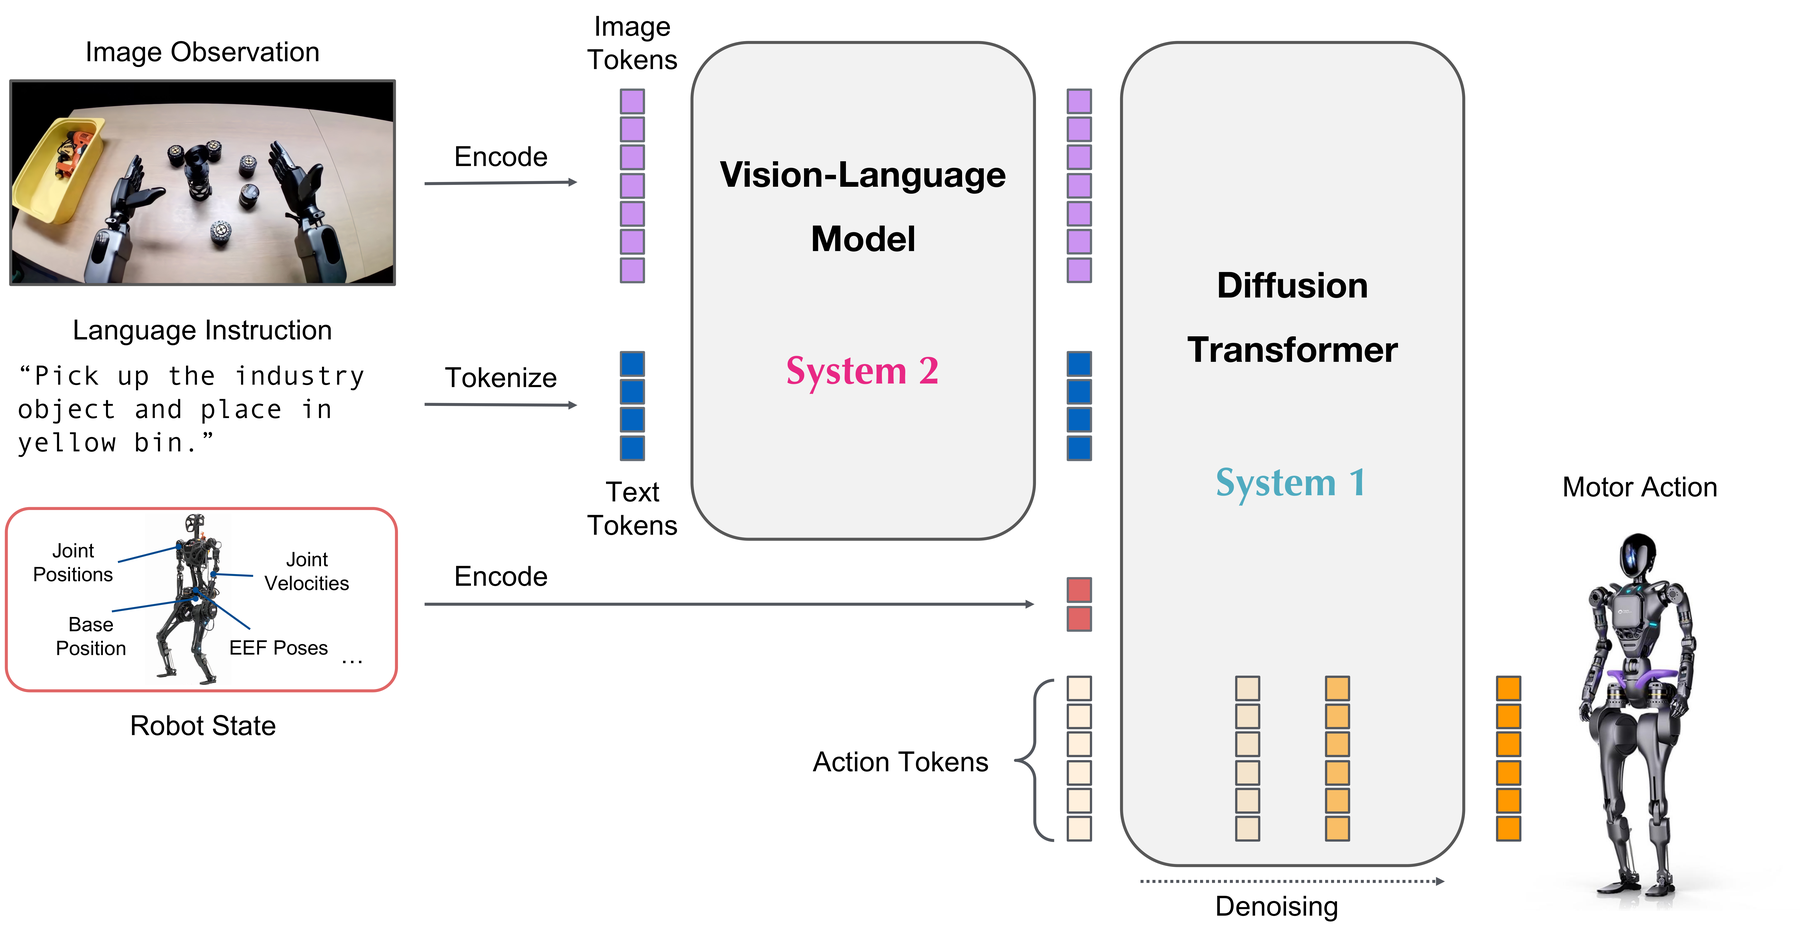
\includegraphics[width=0.95\textwidth]{arch.png}
\caption{Hai khối của GR00T N1.7: VLM hiểu ảnh và câu lệnh; Diffusion Transformer khử nhiễu token hành động dựa trên kết quả đó và trạng thái robot. Nguồn: Isaac-GR00T.}
\label{fig:arch}
\end{figure}

Hình~\ref{fig:arch} là toàn bộ GR00T N1.7 khi đứng riêng. Một lần suy luận đi qua năm bước:
\begin{enumerate}
\item \textbf{Đầu vào:} ảnh camera, có thể kèm một khung quá khứ; câu lệnh; trạng thái khớp của robot.
\item \textbf{VLM:} ảnh và câu lệnh được biến thành một chuỗi vector 2048 chiều đã trộn thông tin ảnh với chữ.
\item \textbf{Action head:} 40 token hành động bắt đầu là nhiễu, cùng 1 token trạng thái, đi qua DiT và hỏi thông tin từ chuỗi vector trên.
\item \textbf{Khử nhiễu 4 lần:} sau mỗi lần, token hành động gần hành động thật hơn.
\item \textbf{Đầu ra:} 40 bước hành động theo đơn vị thật, chia theo nhóm khớp của robot đang dùng.
\end{enumerate}
Đầu ra là gì tuỳ cách khai báo embodiment: với tay máy là góc khớp hoặc pose EEF; với Unitree G1 theo khai báo \code{REAL\_G1} là góc tay, bàn tay, eo. Bảng~\ref{tab:hparams} liệt kê các con số chính.

\begin{table}[htbp]
\centering\small
\caption{Các thông số chính của GR00T N1.7 theo checkpoint phát hành.}
\label{tab:hparams}
\begin{tabular}{L{5cm}L{3cm}L{6.4cm}}
\toprule
\textbf{Thông số} & \textbf{Giá trị} & \textbf{Ý nghĩa}\\
\midrule
Backbone & Cosmos-Reason2-2B & VLM của NVIDIA, kiến trúc Qwen3-VL\\
Số lớp LLM giữ lại & 16 trên 28 & Chỉ dùng nửa đầu mô hình ngôn ngữ\\
Chiều đặc trưng VLM & 2048 & Chiều của mỗi token ảnh hoặc chữ\\
Số lớp DiT & 32 & Số khối Transformer trong action head\\
Chiều token trong DiT & 1536 & 32 head, mỗi head 48 chiều\\
Action chunk & 40 bước & Số bước hành động mỗi lần suy luận\\
Chiều state, action tối đa & 132 & Mọi robot được đệm về cùng chiều này\\
Số bước khử nhiễu & 4 & Số lần chạy DiT mỗi lần suy luận\\
Số embodiment tối đa & 32 & Số ngăn trọng số riêng cho từng loại robot\\
Tổng tham số & khoảng 3,1 tỉ & Backbone 1,5 tỉ; action head 1,6 tỉ\\
Tốc độ trên H100 & 27,9\,ms & Với TensorRT; 85,8\,ms nếu chạy PyTorch thường\\
\bottomrule
\end{tabular}
\end{table}

\subsection{Pipeline của GEAR-SONIC whole-body control}

SONIC là bộ điều khiển toàn thân cho Unitree G1, 42 triệu tham số, huấn luyện bằng học tăng cường trong mô phỏng trên hơn 100 triệu khung hình chuyển động của người. Khi đứng riêng, pipeline của SONIC gồm ba khối:
\begin{enumerate}
\item \textbf{Bộ mã hoá:} nhận một lệnh chuyển động ở một trong ba dạng: chuyển động tham chiếu của robot, tư thế người từ VR hoặc video, hoặc lệnh lai gồm keypoint thân trên cộng chân robot. Mỗi dạng có một bộ mã hoá riêng, tất cả đổ về cùng một motion token 64 chiều.
\item \textbf{Motion token:} vector 64 chiều mô tả ý định chuyển động của toàn thân trong khoảng 1 giây tới. Đây là ngôn ngữ chung của SONIC.
\item \textbf{Bộ giải mã:} nhận token cùng trạng thái robot 10 bước gần nhất, trả về mục tiêu góc cho 29 khớp ở 50\,Hz. Bộ giải mã đã học giữ thăng bằng, nên mọi token đều cho ra chuyển động đứng vững.
\end{enumerate}
Bộ giải mã chạy trên máy tính của robot, lệnh xuống động cơ ở 500\,Hz. Với 14 khớp ngón tay, SONIC không điều khiển; góc ngón đi thẳng xuống bàn tay.

\subsection{Pipeline chung khi ghép GR00T N1.7 với GEAR-SONIC}

Khi ghép, GR00T N1.7 thay thế các bộ mã hoá của SONIC: thay vì người điều khiển VR sinh ra motion token, VLA sinh ra motion token từ ảnh và câu lệnh. Pipeline chung chạy ba tần số:
\begin{enumerate}
\item \textbf{GR00T N1.7, 2,5\,Hz:} nhận ảnh camera đầu, câu lệnh, trạng thái 46 chiều gồm chân, eo, tay, bàn tay và hướng trọng lực; trả về 40 bước, mỗi bước 78 chiều gồm motion token 64 chiều và 14 góc ngón tay.
\item \textbf{Bộ giải mã SONIC, 50\,Hz:} lấy lần lượt từng token trong 40 bước, ghép với trạng thái robot, trả về mục tiêu góc cho 29 khớp thân. 14 góc ngón đi thẳng tới bàn tay.
\item \textbf{Robot hoặc mô phỏng, 500\,Hz:} bộ điều khiển PD bám mục tiêu góc, trả lại trạng thái mới cho cả hai tầng.
\end{enumerate}
Cách ghép này đưa việc giữ thăng bằng và phối hợp chân tay về cho SONIC; GR00T chỉ cần học ý định. Bài báo SONIC cho thấy VLA dự đoán motion token đạt tỉ lệ thành công 68\% so với 27\% khi dự đoán trực tiếp tư thế; ở nhiệm vụ bỏ lon vào thùng rác, khác biệt là 60\% so với 0\%.

Trong dự án của nhóm, vì chưa có dữ liệu motion token, đường chạy hiện dùng khai báo \code{REAL\_G1}: GR00T trả về góc tay, bàn tay, eo; bộ điều khiển bám các góc này ở 50\,Hz và giữ chân ở tư thế đứng. Đây là bước trung gian trước khi chuyển sang pipeline chung đầy đủ.

\section{Xử lý ảnh}

Ảnh đi qua hai bước trước khi vào mạng. Bước tiền xử lý thu ảnh về cạnh ngắn 256 điểm ảnh, cắt giữ 95\% ở giữa, và không ép về hình vuông; khi huấn luyện, phép cắt là ngẫu nhiên, thêm xoay nhẹ và đổi màu để mô hình quen với nhiều điều kiện. Bước mã hoá của Qwen3-VL cắt ảnh thành các ô $16 \times 16$, mỗi ô thành một token 1024 chiều, rồi 24 lớp Transformer cho các ô trao đổi thông tin. Sau đó projector gộp 4 ô kề nhau thành một token và chiếu về 2048 chiều. Vì mỗi ô đã chứa thông tin của các ô xung quanh, gộp 4 gần như không mất thông tin nhưng giảm 4 lần chi phí. Một ảnh $256 \times 256$ chỉ tốn 64 token trong mô hình ngôn ngữ. Bộ mã hoá ảnh mặc định đóng băng khi fine-tune.

\begin{figure}[htbp]
\centering
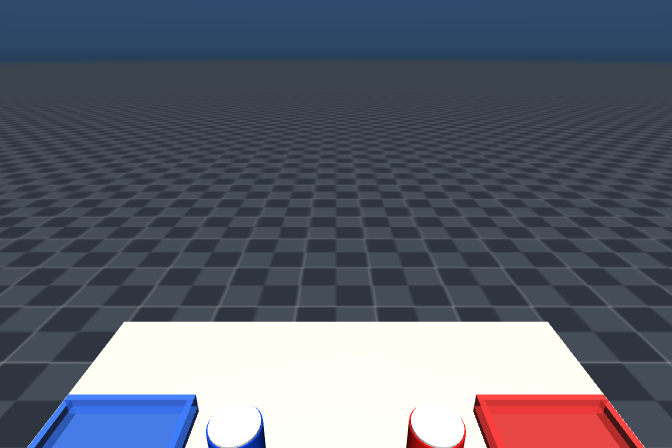
\includegraphics[width=0.5\textwidth]{ego.png}
\caption{Ảnh camera \code{ego\_view} của Unitree G1 trong mô phỏng của nhóm, đầu vào ảnh cho GR00T N1.7.}
\label{fig:ego}
\end{figure}

\section{Xử lý image + text đầu vào}

Câu lệnh được đưa về chữ thường và bỏ dấu câu, rồi ghép với các ảnh thành một lượt hội thoại theo mẫu của Qwen3-VL: ảnh trước, chữ sau. Mô hình ngôn ngữ đọc chuỗi này; qua các lớp attention, token chữ ``red'' gom thông tin từ các token ảnh có vật màu đỏ và ngược lại. GR00T chỉ giữ 16 lớp đầu trong 28 lớp của mô hình ngôn ngữ và không sinh chữ: các lớp giữa cho đặc trưng bám ảnh tốt hơn cho điều khiển, và tiết kiệm tính toán. Đầu ra là chuỗi vector 2048 chiều kèm một mặt nạ đánh dấu token nào là ảnh, token nào là chữ. Toàn bộ backbone đóng băng khi fine-tune; giữa backbone và DiT có thêm một khối nhỏ gồm 4 lớp self-attention được huấn luyện để ``dịch'' đặc trưng cho phù hợp với action head.

\section{Sinh hành động: Diffusion Action Head}

Action head làm việc với 41 token: 1 token trạng thái robot và 40 token hành động. Token trạng thái do một MLP riêng của từng embodiment tạo ra. Token hành động ban đầu là nhiễu, được ghép thêm thông tin ``đang ở mức nhiễu nào'' và vị trí bước thứ mấy trong chunk.

32 khối DiT xử lý 41 token này theo chu kỳ 4 khối: khối thứ nhất cross-attention tới token chữ, khối thứ hai self-attention giữa 41 token, khối thứ ba cross-attention tới token ảnh, khối thứ tư self-attention. Tách riêng lượt hỏi chữ và lượt hỏi ảnh giúp câu lệnh không bị ``chìm'' giữa hàng trăm token ảnh; đây là thay đổi kiến trúc thực sự của N1.7 so với N1.6. Self-attention giữa 40 token hành động giúp chúng thống nhất với nhau thành một chuyển động liên tục.

Đầu ra của DiT qua một MLP riêng của embodiment để thành ``hướng đi'' cho 40 bước hành động. Mô hình cộng hướng đi này vào token hành động, lặp lại 4 lần, và thu được chunk hành động sạch. Backbone chỉ chạy một lần mỗi lần quan sát; 4 vòng lặp chỉ chạy lại action head nên suy luận nhanh.

\section{Trạng thái robot và cách ghi hành động}

Trạng thái robot gồm các nhóm khớp, mỗi nhóm được chuẩn hoá về đoạn $[-1, 1]$ theo thống kê của embodiment, nối lại và đệm về 132 chiều. Khi huấn luyện, có xác suất 20\% toàn bộ trạng thái bị thay bằng 0 để mô hình phải nhìn ảnh thay vì chỉ dựa vào góc khớp.

Hành động được khai báo theo từng nhóm: tuyệt đối hay relative, ở không gian khớp hay EEF. Với nhóm relative, dữ liệu huấn luyện được đổi thành độ dời so với trạng thái hiện tại; khi chạy, mô hình cộng ngược độ dời lên trạng thái để trả về mục tiêu tuyệt đối. Mỗi embodiment có một chỉ số từ 0 đến 31 để chọn đúng ngăn trọng số trong các MLP mã hoá và giải mã. Phần hiểu ảnh, chữ và DiT dùng chung cho mọi robot; chỉ phần ``phiên dịch'' sang không gian khớp của từng robot là riêng.

\begin{table}[htbp]
\centering\footnotesize
\caption{Hai cách khai báo Unitree G1 trong GR00T N1.7 mà nhóm đã dùng.}
\label{tab:g1emb}
\begin{tabular}{L{2.8cm}L{5.9cm}L{5.9cm}}
\toprule
\textbf{Thuộc tính} & \textbf{REAL\_G1} & \textbf{UNITREE\_G1\_SONIC}\\
\midrule
Ảnh & \code{ego\_view}, khung hiện tại và khung 20 bước trước & \code{ego\_view}, khung hiện tại\\
Trạng thái & Pose 2 cổ tay, 2 bàn tay, 2 cánh tay, eo: 49 chiều & 2 chân, eo, 2 cánh tay, 2 bàn tay, hướng trọng lực: 46 chiều\\
Hành động & Như trạng thái, thêm chiều cao thân và lệnh di chuyển: 53 chiều; cổ tay và cánh tay ghi relative & Motion token 64 chiều và 14 khớp ngón tay: 78 chiều\\
Có sẵn trong checkpoint & Có, kèm thống kê chuẩn hoá & Không, phải fine-tune trên dữ liệu SONIC\\
\bottomrule
\end{tabular}
\end{table}

\section{Triển khai và giao tiếp giữa các thành phần}

Isaac-GR00T tách mô hình và robot thành hai tiến trình nói chuyện qua mạng. Policy server chạy trên máy có GPU, cần tối thiểu 16\,GB bộ nhớ. Policy client chạy trên robot hoặc máy mô phỏng, gửi ảnh, trạng thái, câu lệnh và nhận lại action chunk. Robot thực thi 8 đến 16 bước đầu của chunk rồi hỏi lại. Bộ giải mã SONIC chạy trên máy robot dưới dạng C++ hoặc ONNX, không cần GPU.

\begin{figure}[htbp]
\centering
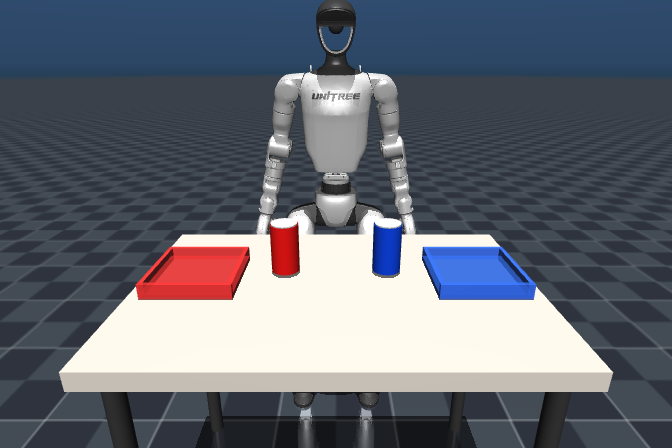
\includegraphics[width=0.5\textwidth]{front.png}
\caption{Cảnh mô phỏng MuJoCo của nhóm: Unitree G1, bàn, lon Coca-Cola, lon Pepsi và hai khay phân loại.}
\label{fig:front}
\end{figure}

% ---------------------------------------------------------------------
\chapter{DỮ LIỆU VÀ PHƯƠNG PHÁP HUẤN LUYỆN}
% ---------------------------------------------------------------------

\section{Cấu trúc dữ liệu vào và ra}

\subsection{Dữ liệu khi chạy và fine-tune riêng GR00T N1.7}

Khi chạy, mô hình nhận ba thứ: ảnh từ một hoặc nhiều camera, có thể kèm khung quá khứ; trạng thái robot theo từng nhóm khớp; và câu lệnh. Mô hình trả về từng nhóm hành động theo đơn vị thật, 40 bước.

Khi fine-tune, dữ liệu là các episode demo theo định dạng LeRobot v2: mỗi khung có ảnh, trạng thái, hành động và câu lệnh; kèm tệp \code{modality.json} cho biết đoạn nào của vector trạng thái và hành động là nhóm khớp nào, camera tên gì, câu lệnh ở cột nào. Nhờ tệp này, cùng một mã nguồn đọc được dữ liệu của mọi robot. Hành động trong demo là thứ mô hình học bắt chước, nên hành động phải cùng định nghĩa với thứ robot sẽ thực thi lúc chạy. Với khai báo \code{REAL\_G1} của nhóm, trạng thái 49 chiều và hành động 53 chiều đều là pose cổ tay, góc tay, bàn tay, eo; dataset được sinh ở 25\,Hz.

\subsection{Dữ liệu khi ghép với whole-body control}

Khi ghép với SONIC, chỉ đầu ra đổi: mỗi khung demo phải có nhãn hành động 78 chiều gồm motion token 64 chiều và 14 góc ngón tay, và trạng thái 46 chiều gồm chân, eo, tay, bàn tay, hướng trọng lực. Ảnh và câu lệnh không đổi. Có hai tầng dữ liệu:
\begin{itemize}
\item \textbf{Dữ liệu của SONIC:} 700 giờ bắt chuyển động của người, huấn luyện tốn 21 nghìn giờ GPU. Nhóm dùng checkpoint có sẵn, không huấn luyện lại.
\item \textbf{Dữ liệu fine-tune VLA:} NVIDIA thu bằng teleoperation VR: người điều khiển làm mẫu, SONIC bám theo trên robot, hệ thống ghi lại ảnh, trạng thái và motion token đang dùng, nên nhãn token có sẵn. Khuyến nghị 50 đến 100 demo cho một nhiệm vụ, mỗi demo làm đúng ngay lần đầu. Benchmark thật của NVIDIA với quy trình này đạt 73,6\% ở nhiệm vụ đi tới bàn và nhấc vật, 66,7\% ở nhiệm vụ bỏ lon vào thùng rác.
\end{itemize}
Với nhóm, dữ liệu mô phỏng tự sinh không có token sẵn, phải chạy bộ mã hoá của SONIC trên quỹ đạo khớp để tính. Nhóm đã bọc bộ mã hoá này nhưng chưa kiểm chứng xong cách ghép vector đầu vào, nên dữ liệu hiện tại vẫn theo khai báo \code{REAL\_G1}.

\section{Tiền huấn luyện và nguồn dữ liệu}

GR00T N1.7 được tiền huấn luyện trên 21,6 triệu mẫu từ 13 dataset, gồm dữ liệu robot thật của nhiều loại tay máy và robot hình người, dữ liệu mô phỏng, và 20 nghìn giờ video góc nhìn thứ nhất của người. Vì hành động ghi ở EEF dưới dạng relative nên video người và dữ liệu robot dùng chung một cách ghi, mô hình học được thao tác từ video người rồi chuyển sang robot. Đây là lý do NVIDIA nêu cho việc N1.7 khái quát tốt hơn N1.6.

Ngoài checkpoint gốc, NVIDIA phát hành bốn checkpoint đã fine-tune cho các benchmark LIBERO, DROID và SimplerEnv. Với Unitree G1, checkpoint gốc có sẵn thống kê cho embodiment \code{REAL\_G1} nhưng không có cho \code{UNITREE\_G1\_SONIC}.

\section{Tiền xử lý và khai báo embodiment}

Ảnh, câu lệnh và trạng thái được xử lý như mô tả ở chương 3. Các tham số tiền xử lý được ghi trong checkpoint nên khi chạy không cần khai báo lại. Với robot mới, người dùng viết một tệp cấu hình embodiment gồm: tên camera và khung quá khứ dùng, danh sách nhóm trạng thái, danh sách nhóm hành động kèm kiểu ghi, và cột câu lệnh. Sau đó chạy một lệnh tính thống kê chuẩn hoá cho dataset rồi fine-tune.

Nhóm gặp một điểm cần lưu ý: nếu fine-tune dữ liệu mô phỏng dưới tag \code{REAL\_G1} đã có trong checkpoint, mã nguồn giữ nguyên thống kê của robot thật và bỏ qua thống kê của dữ liệu mình. Cách giải quyết là đăng ký dưới tag \code{NEW\_EMBODIMENT}; đổi lại ngăn trọng số riêng của embodiment phải học từ đầu.

\section{Mục tiêu huấn luyện}

Action head học theo flow matching. Với mỗi mẫu, mã nguồn trộn hành động thật với nhiễu theo một tỉ lệ ngẫu nhiên, lệch về phía nhiều nhiễu, rồi bắt mô hình đoán ``hướng đi'' từ điểm trộn đó về hành động thật. Sai số là bình phương giữa hướng đoán và hướng đúng, chỉ tính trên phần hành động thật, bỏ phần đệm. Backbone đóng băng nên không có sai số phụ nào khác. Tối ưu bằng AdamW, learning rate $10^{-4}$, batch 32 đến 64, mặc định 10 nghìn bước. NVIDIA khuyến nghị GPU 40\,GB trở lên để fine-tune.

\section{Chiến lược fine-tune}

Mặc định của Isaac-GR00T là đóng băng toàn bộ backbone và huấn luyện toàn bộ action head: 4 lớp self-attention cầu nối, 32 lớp DiT, và các MLP mã hoá, giải mã của embodiment. Tổng cộng khoảng 1,6 tỉ trên 3,1 tỉ tham số được cập nhật. Có cờ để mở thêm bộ mã hoá ảnh hoặc vài lớp trên cùng của mô hình ngôn ngữ khi cần, nhưng tốn GPU lớn hơn nhiều. Mã nguồn không có sẵn LoRA cho backbone; nếu muốn chỉnh phần hiểu ảnh một cách nhẹ, ví dụ để phân biệt tốt hơn hai lon gần giống nhau, LoRA là hướng nhóm phải tự bổ sung.

NVIDIA khuyến nghị kiểm tra fine-tune bằng open-loop: vẽ hành động dự đoán chồng lên hành động ghi sẵn, theo dõi sai số giảm dần qua các checkpoint, và tự lập baseline thay vì so với một ngưỡng cố định.

% ---------------------------------------------------------------------
\chapter{SO SÁNH VỚI CÁC MÔ HÌNH CÙNG LOẠI}
% ---------------------------------------------------------------------

\section{GR00T N1.7 và $\pi_{0.5}$}

$\pi_{0.5}$ của Physical Intelligence là mô hình VLA được nhắc tới nhiều nhất cùng thời điểm. Hai mô hình giống nhau ở khung chung: một VLM khoảng 3 tỉ tham số đóng vai trò backbone, một action expert sinh action chunk bằng flow matching. Khác biệt nằm ở mục tiêu và cách dùng dữ liệu, tóm tắt ở Bảng~\ref{tab:pi05}.

\begin{table}[htbp]
\centering\small
\caption{So sánh GR00T N1.7 và $\pi_{0.5}$ ở các điểm quan trọng với nhóm.}
\label{tab:pi05}
\begin{tabular}{L{3.4cm}L{5.5cm}L{5.5cm}}
\toprule
\textbf{Tiêu chí} & \textbf{GR00T N1.7} & \textbf{$\pi_{0.5}$}\\
\midrule
Robot mục tiêu & Robot hình người và nhiều loại tay máy; có đường riêng cho whole-body control & Tay máy cố định và robot di động hai tay; không có whole-body control\\
Backbone & Cosmos-Reason2-2B, giữ 16 lớp, đóng băng & PaliGemma 3B, được huấn luyện cùng\\
Suy luận cấp cao & Không; mô hình đi thẳng từ câu lệnh tới hành động & Có: mô hình tự sinh mô tả bước con bằng chữ trước, rồi sinh hành động theo bước con đó\\
Dữ liệu tiền huấn luyện & Dữ liệu robot nhiều loại, mô phỏng, 20 nghìn giờ video người & Khoảng 400 giờ robot di động trong hơn 100 căn nhà, cộng dữ liệu tay máy, dữ liệu web và nhãn ngôn ngữ\\
Điểm mạnh đã chứng minh & Fine-tune nhanh cho robot mới; chạy được trên GPU 16\,GB và Jetson; giao diện với SONIC & Khái quát sang nhà chưa từng thấy, làm nhiệm vụ dài như dọn bếp, dọn giường\\
Giấy phép & Apache 2.0 và NVIDIA Open Model License, dùng thương mại được & Mã và trọng số mở qua openpi, giấy phép Apache 2.0\\
Công cụ triển khai & Policy server, ONNX, TensorRT, tích hợp LeRobot & Policy server, mã tham chiếu\\
\bottomrule
\end{tabular}
\end{table}

\textbf{GR00T N1.7 tốt hơn ở đâu.} Nó là lựa chọn duy nhất trong hai mô hình có đường đi hoàn chỉnh cho robot hình người: dữ liệu, tag embodiment, bộ điều khiển toàn thân và benchmark thật trên Unitree G1. Việc đóng băng backbone và tách ngăn trọng số theo embodiment làm fine-tune rẻ và ổn định. Công cụ triển khai đầy đủ hơn.

\textbf{GR00T N1.7 chưa bằng ở đâu.} Nó không có bước suy luận cấp cao: khi nhiệm vụ dài và cần chia thành nhiều bước, $\pi_{0.5}$ tự nói ra bước con rồi làm, còn GR00T phải dựa vào câu lệnh ngắn và dữ liệu demo. Kết quả khái quát sang môi trường lạ của GR00T được công bố ít hơn và chủ yếu trên benchmark mô phỏng. Backbone đóng băng cũng có nghĩa phần hiểu ảnh không học được gì mới từ dữ liệu của mình nếu không mở thêm cờ tốn tài nguyên.

\section{So với các mô hình khác}

OpenVLA rời rạc hoá hành động thành token chữ nên chậm và chuyển động giật; GR00T và $\pi$ sinh hành động liên tục bằng flow matching, mượt hơn nhiều. Các mô hình đóng như RT-2 không có trọng số mở. Về phía WBC, các bộ điều khiển tách rời trước SONIC chỉ nhận tư thế thân trên hoặc keypoint; SONIC là bộ đầu tiên đưa ra một không gian token chung cho teleoperation, planner và VLA.

\section{So với policy lập trình sẵn hoặc policy học một nhiệm vụ}

Trong dự án của nhóm, quỹ đạo lập trình sẵn chỉ chịu được lon lệch 1 đến 2\,cm vì chạy mù theo điểm cố định; mỗi vật thể mới, mỗi vị trí mới đều phải viết lại. Một policy học một nhiệm vụ bằng imitation learning thông thường cần hàng trăm demo cho đúng cảnh đó và không nghe lệnh. VLA như GR00T hơn ở ba điểm: nghe được câu lệnh nên một mô hình làm nhiều nhiệm vụ; phần hiểu ảnh đã học từ hàng chục nghìn giờ dữ liệu nên chỉ cần vài chục demo để thích nghi; và cách ghi hành động relative giúp chịu được vật thể đổi vị trí. Đổi lại, VLA cần GPU khi chạy, và chất lượng phụ thuộc nhiều vào dữ liệu fine-tune.

\section{Nhược điểm hiện tại của GR00T N1.7}

\begin{itemize}
\item \textbf{Chưa dùng ngay được cho robot mới.} Với robot ngoài danh sách tiền huấn luyện, phải có dữ liệu demo và fine-tune; zero-shot chỉ hoạt động trên các embodiment có sẵn.
\item \textbf{Không có suy luận nhiều bước.} Mô hình chỉ nhìn hai khung ảnh và một câu lệnh, không nhớ dài, không tự chia nhiệm vụ.
\item \textbf{Thiếu dữ liệu và checkpoint cho whole-body control.} Tag \code{UNITREE\_G1\_SONIC} tồn tại nhưng NVIDIA chưa công bố dataset hay checkpoint fine-tune; muốn dùng phải tự thu dữ liệu bằng teleoperation VR hoặc tự tính token.
\item \textbf{Phụ thuộc thống kê chuẩn hoá.} Sai thứ tự khớp, sai hệ toạ độ hoặc sai thống kê là mô hình cho quỹ đạo vô nghĩa, và không có cảnh báo. Nhóm đã mất thời gian dò lại quy ước thứ tự ngón tay và hệ toạ độ cổ tay vì tài liệu không ghi.
\item \textbf{Cần GPU.} Tối thiểu 16\,GB để chạy, 40\,GB để fine-tune; backbone Cosmos-Reason2 là mô hình gated trên Hugging Face, phải xin quyền.
\item \textbf{Tỉ lệ thành công thật còn thấp.} Ngay trên benchmark của NVIDIA, gắp vật với SONIC đạt khoảng 70\%, lỗi chủ yếu là gắp trượt.
\end{itemize}

% ---------------------------------------------------------------------
\chapter{KẾT QUẢ THỬ NGHIỆM CỦA NHÓM}
% ---------------------------------------------------------------------
Nhóm thử GR00T N1.7 trên mô phỏng MuJoCo với Unitree G1 43 khớp, nhiệm vụ gắp lon Coca-Cola bỏ vào khay đỏ và lon Pepsi bỏ vào khay xanh. Máy cục bộ không có GPU nên mô hình chạy trên Google Colab, mô phỏng chạy cục bộ và nối qua mạng. Ba việc đã làm như sau.

\section{Nối GR00T N1.7 với bộ điều khiển toàn thân}

\begin{itemize}
\item Dựng đường chạy ba tần số: GR00T suy luận 2,5 đến 5\,Hz, bộ điều khiển toàn thân 50\,Hz, mô phỏng vật lý 500\,Hz.
\item Viết policy server chạy mô hình thật trên Colab và client gửi ảnh, trạng thái, câu lệnh từ mô phỏng. Server lỗi thì robot giữ tư thế, không âm thầm chạy quỹ đạo giả.
\item Viết adapter đổi trạng thái mô phỏng sang khai báo \code{REAL\_G1} và đổi hành động của mô hình thành 43 mục tiêu góc, nội suy lên 50\,Hz.
\item Bọc bộ giải mã và bộ mã hoá của SONIC dưới dạng ONNX. Bộ mã hoá chưa kiểm chứng xong nên đường chạy hiện dùng chế độ bám góc khớp, chân giữ tư thế đứng.
\item Phát hiện quan trọng khi chạy zero-shot: camera trong mô phỏng nghiêng 24 độ chỉ thấy sàn và mép lon, ảnh lệch hẳn dữ liệu huấn luyện, robot giơ tay lung tung. Sau khi chỉnh camera về 50 độ, hành vi hợp lý hơn.
\end{itemize}

\section{Tự sinh dữ liệu demo}

Không có dataset công khai nào đúng bài toán, nên nhóm tự sinh dữ liệu trong mô phỏng theo định dạng LeRobot.

\begin{itemize}
\item Phiên bản đầu dùng quỹ đạo lập trình sẵn, lon lệch trong ô $4 \times 4$\,cm: 100 episode huấn luyện, 40 episode kiểm tra. Hạn chế: hành động gần như không phụ thuộc vị trí lon nên mô hình có thể học thuộc quỹ đạo thay vì học nhìn.
\item Phiên bản hai dùng động học ngược giải theo từng episode: lon đặt ngẫu nhiên trong vùng $11 \times 16$\,cm, đứng hoặc nằm với hướng bất kỳ; có kiểm tra va chạm, tự chọn đường vòng khi bị chắn. Bộ lập kế hoạch thành công 36/36 với lon đứng, 78\% với lon nằm bên tay phải và 69\% bên tay trái. Chỉ giữ episode thành công và phát lại được.
\item Có công cụ kiểm tra định dạng, phát lại hành động qua mô phỏng, và vẽ phân bố vị trí lon để bảo đảm tập kiểm tra không trùng tập huấn luyện.
\end{itemize}

\section{Fine-tune trên Google Colab}

Nhóm fine-tune từ checkpoint gốc trên GPU L4, batch 32, 5000 bước, dữ liệu phiên bản đầu, khai báo dưới tag \code{NEW\_EMBODIMENT}. Kết quả open-loop ở Bảng~\ref{tab:openloop}.

\begin{table}[htbp]
\centering\small
\caption{Sai số open-loop của checkpoint 5000 bước, đơn vị hành động chuẩn hoá. MAE 0,005 tương đương khoảng 0,3 độ.}
\label{tab:openloop}
\begin{tabular}{llrr}
\toprule
\textbf{Tập} & \textbf{Lon} & \textbf{MSE trung bình} & \textbf{MAE trung bình}\\
\midrule
Huấn luyện & Coca, 20 episode & 0,000303 & 0,00509\\
Huấn luyện & Pepsi, 20 episode & 0,000264 & 0,00509\\
Kiểm tra & Coca, 20 episode & 0,000320 & 0,00537\\
Kiểm tra & Pepsi, 20 episode & 0,000267 & 0,00516\\
\bottomrule
\end{tabular}
\end{table}

Nhận định: chênh lệch giữa tập huấn luyện và kiểm tra khoảng 3\%, sai số đều giữa các episode, nên mô hình không học thuộc trong vùng đã thử. Nhưng vì dữ liệu phiên bản đầu ít phụ thuộc vị trí lon, kết quả này chưa chứng minh mô hình biết nhìn lon. Việc đang làm: sinh khoảng 400 episode từ dữ liệu phiên bản hai, fine-tune lại, và chạy closed-loop bằng công cụ đánh giá đã viết, đo tỉ lệ gắp thành công theo vị trí lon.

\section{Bài học rút ra}

\begin{itemize}
\item Quy trình fine-tune của Isaac-GR00T chạy được trên Colab với GPU L4, khoảng vài giờ cho 5000 bước; không cần cụm GPU lớn cho bài toán nhỏ.
\item Phần tốn công nhất không phải huấn luyện mà là khớp dữ liệu với mô hình: thứ tự khớp, hệ toạ độ, thống kê chuẩn hoá, góc camera. Sai một chỗ là mô hình vô dụng mà không báo lỗi.
\item Dữ liệu demo phải đa dạng vị trí và hướng vật thể; dữ liệu chạy mù cho sai số thấp nhưng không dạy được mô hình nhìn.
\item Muốn dùng whole-body control thật sự phải giải quyết nhãn motion token; đây là điểm nghẽn để chuyển từ chế độ bám góc khớp sang SONIC đầy đủ.
\end{itemize}

% ---------------------------------------------------------------------
\chapter{KẾT LUẬN VÀ ĐỀ XUẤT}
% ---------------------------------------------------------------------
GR00T N1.7 là mô hình VLA mở phù hợp nhất hiện nay cho robot hình người nhờ đường đi hoàn chỉnh từ dữ liệu tới bộ điều khiển toàn thân, công cụ triển khai tốt và giấy phép dùng thương mại. So với $\pi_{0.5}$, nó thua ở suy luận nhiều bước và bằng chứng khái quát ngoài đời, nhưng hơn ở hỗ trợ robot hình người và chi phí fine-tune. Nhóm đã nối được mô hình với mô phỏng và bộ điều khiển toàn thân, tự sinh được dữ liệu, và fine-tune thành công về mặt sai số open-loop.

Đề xuất bước tiếp theo, theo thứ tự ưu tiên:
\begin{enumerate}
\item Chạy closed-loop với checkpoint fine-tune trên dữ liệu phiên bản hai để có tỉ lệ thành công thật, đây là con số cần có trước khi quyết định đi tiếp.
\item Hoàn thiện bộ mã hoá SONIC để dữ liệu có nhãn motion token, chuyển sang tag \code{UNITREE\_G1\_SONIC} và có thăng bằng thật.
\item Nếu mô hình vẫn không phân biệt được hai lon, thử mở bộ mã hoá ảnh hoặc bổ sung LoRA cho backbone, cần GPU 80\,GB.
\item Theo dõi phiên bản GR00T tiếp theo và openpi; nếu $\pi$ bổ sung whole-body control thì cần đánh giá lại lựa chọn.
\end{enumerate}

% ---------------------------------------------------------------------
\renewcommand{\bibname}{TÀI LIỆU THAM KHẢO}
\begin{thebibliography}{99}
\addcontentsline{toc}{chapter}{Tài liệu tham khảo}
\bibitem{isaacgr00t} NVIDIA, ``Isaac GR00T N1.7,'' kho mã nguồn \url{https://github.com/NVIDIA/Isaac-GR00T}, commit 51d4c89, 2026.
\bibitem{hfcard} NVIDIA, ``GR00T-N1.7-3B,'' model card, \url{https://huggingface.co/nvidia/GR00T-N1.7-3B}, 2026.
\bibitem{gr00tn1} J. Bjorck và cộng sự, ``GR00T N1: An Open Foundation Model for Generalist Humanoid Robots,'' arXiv:2503.14734, 2025.
\bibitem{sonic} NVIDIA GEAR Lab, ``SONIC: Supersizing Motion Tracking for Natural Humanoid Whole-Body Control,'' arXiv:2511.07820, 2025; \url{https://nvlabs.github.io/GEAR-SONIC/}.
\bibitem{wbc} NVlabs, ``GR00T-WholeBodyControl,'' \url{https://nvlabs.github.io/GR00T-WholeBodyControl/}, 2026.
\bibitem{pi05} Physical Intelligence, ``$\pi_{0.5}$: a Vision-Language-Action Model with Open-World Generalization,'' arXiv:2504.16054, 2025.
\bibitem{pi0} K. Black và cộng sự, ``$\pi_0$: A Vision-Language-Action Flow Model for General Robot Control,'' arXiv:2410.24164, 2024.
\bibitem{openvla} M. J. Kim và cộng sự, ``OpenVLA: An Open-Source Vision-Language-Action Model,'' CoRL, 2024.
\bibitem{dp} C. Chi và cộng sự, ``Diffusion Policy: Visuomotor Policy Learning via Action Diffusion,'' RSS, 2023.
\bibitem{flow} Y. Lipman và cộng sự, ``Flow Matching for Generative Modeling,'' ICLR, 2023.
\bibitem{lerobot} Hugging Face, ``LeRobot,'' \url{https://github.com/huggingface/lerobot}.
\bibitem{project} Nguyễn Duy Hoàng, dự án GEAR-SONIC-GR00T-N1.7: README.md, MEMO\_VLA\_FINETUNE.md, mã nguồn thư mục bridge, sim, tools, 2026.
\end{thebibliography}

\end{document}
